\chapter{Analisis}
\label{chap:analsa}

\section{Kondisi IDE UNPAR dibandingkan dengan Moodle Standar}
\label{sec:Kondisi IDE UNPAR} 
IDE UNPAR sudah mengalami perubahan dan penyesuaian agar dapat digunakan, perubahan dan penyesuaian tersebut harus diterapkan juga didalam Moodle mobile. Perubahan dan penyesuain yang dimaksud adalah perbedaan dari tampilan dan fitur IDE UNPAR yang tidak ada dalam situs Moodle standar dan dapat dilihat oleh peneliti. Perubahan dan penyesuaian terhadap IDE UNPAR akan adalah sebagai berikut\cite{IDEUNPAR}.

\subsubsection {Penggunaan tema Snap Moodle}
	Tampilan IDE UNPAR sudah berbeda dari tampilan standar milik Moodle. perubahan ini terlihat ketika memeriksa elemen dari IDE UNPAR pada baigan HTML \textit{tag}. Salah satu \textit{tag link} pada \textit{tag head} IDE UNPAR mengarahkan file \texttt{styles.php} pada direkotori bernama \textit{snap}. Ketika mencari Snap pada forum \textit{plugin} Moodle ditemukan tema dengan tampilan seperti Gambar \ref{fig:snap-personal} yang menyerupai tampilan IDE. Dengan beberapa perbedaan seperti pada warna dan \textit{progress bar} dibawah \textit{activity card}. Kemiripan juga dapat dilihat dengan membandingkan Gambar \ref{fig:snap-personal} dengan Gambar \ref{fig:snap-ide}

\begin{figure}[H] 
	\centering  
	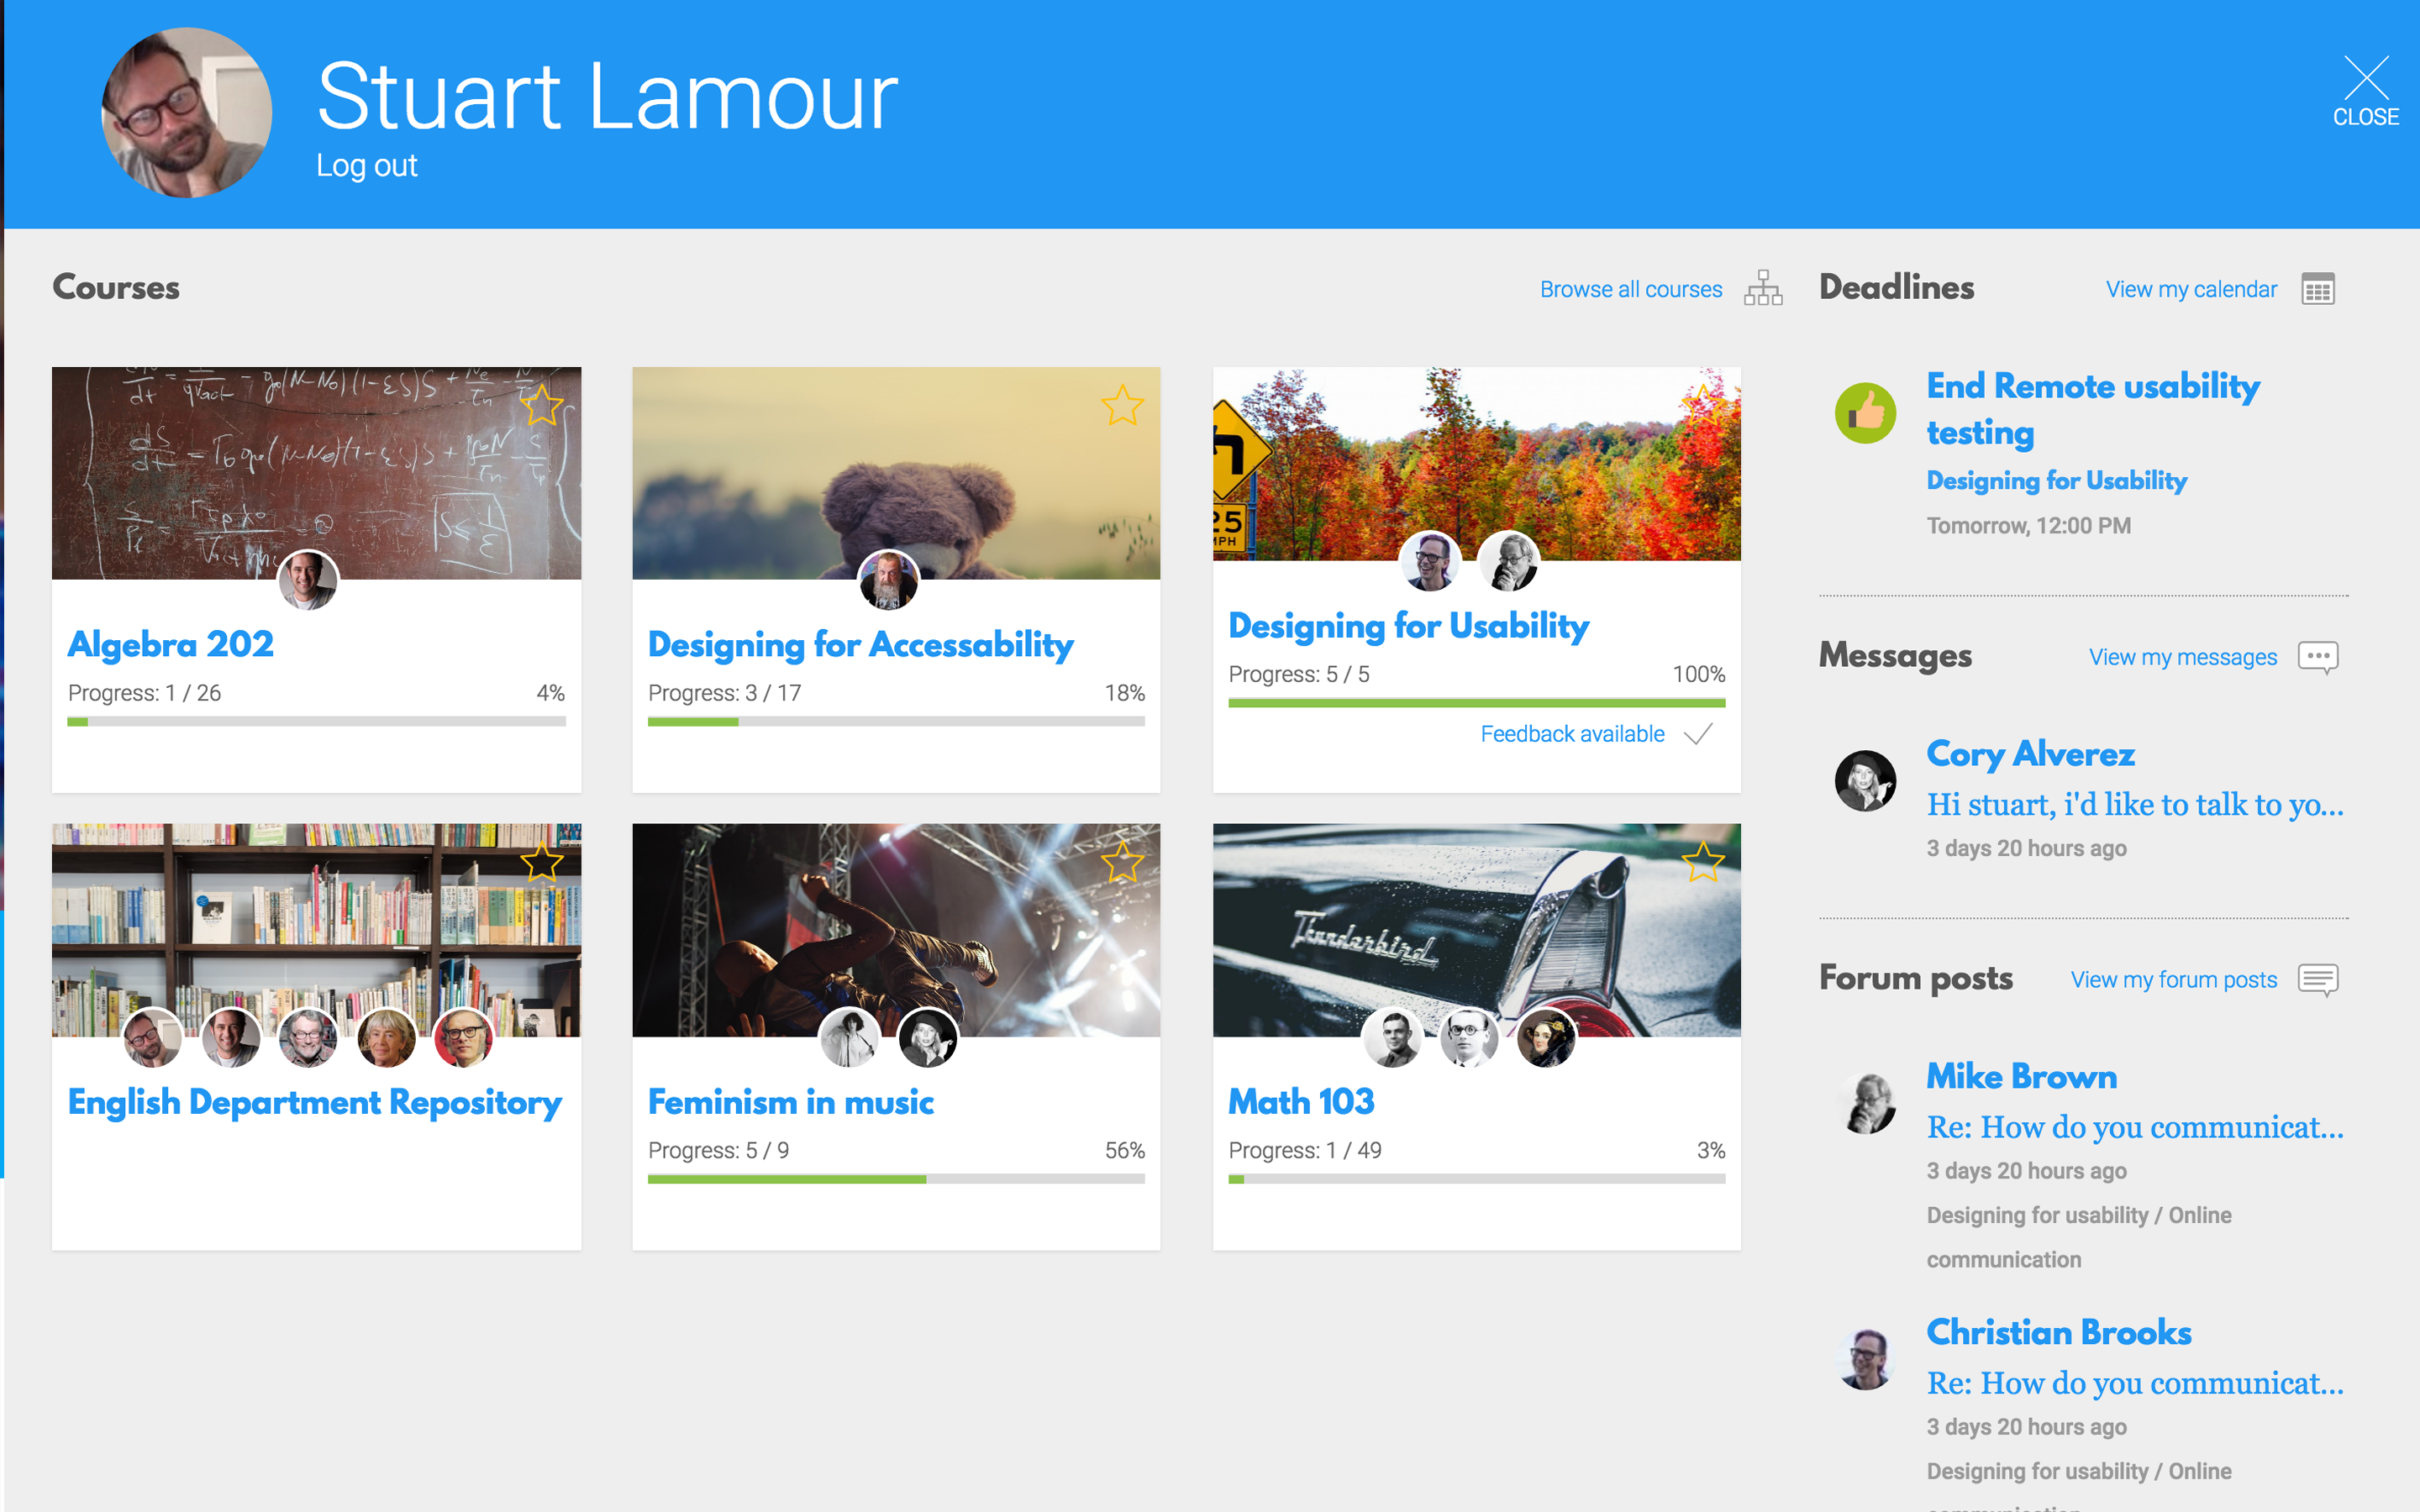
\includegraphics[scale=0.16]{snap-personalmenu.png}  
	\caption[Tampilan dashboard tema Snap] {Tampilan tema Snap} 
	\label{fig:snap-personal} 
\end{figure} 

\begin{figure}[H] 
	\centering  
	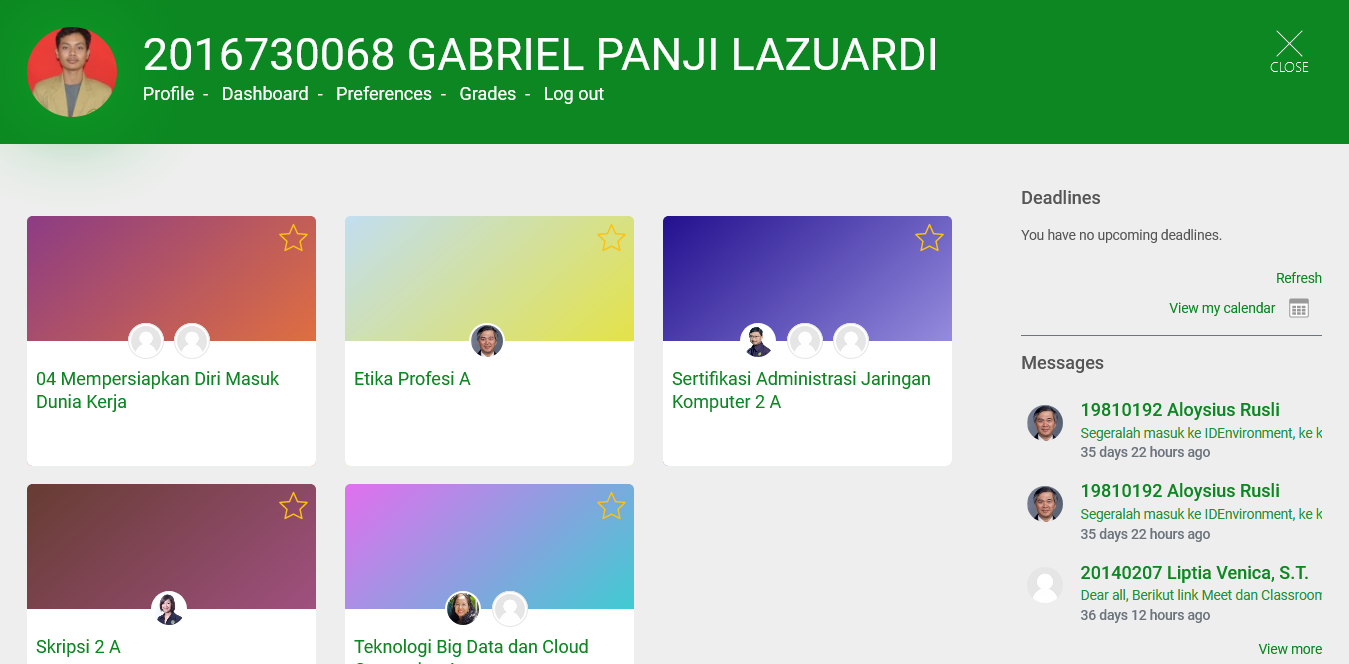
\includegraphics[scale=0.3]{snap-ide.png}  
	\caption[Tampilan dashboard IDE UNPAR] {Tampilan IDE UNPAR} 
	\label{fig:snap-ide} 
\end{figure} 
\subsubsection {Mata kuliah dan peserta mata kuliah}
IDE UNPAR sudah digunakan dalam proses belajar mengajar selama perkuliahan di UNPAR, sehingga IDE UNPAR sudah terisi dengan data dosen-dosen dan mata kuliah yang mereka ajarkan. Beserta dengan data-data tersebut IDE UNPAR juga sudah terisi dengan data-data mahasiswa aktif di UNPAR.
\subsubsection {\textit{Banner} pada halaman utama}
IDE UNPAR menggunakan sebuah korsel untuk menunjukkan nama situs dan pengumuman seperti pada Gambar \ref{fig:korsel-unpar}. Korsel yang digunakan oleh IDE UNPAR adalah bawaan juga dari tema Snap yang digunakan.
\begin{figure}[H] 
	\centering  
	
\includegraphics[scale=0.2]{korsel-unpar.png}  
	\caption[Korsel pada halaman utama] {Korsel pada halaman utama IDE UNPAR} 
	\label{fig:korsel-unpar} 
\end{figure}
\subsubsection {Bagian panduan digital}
IDE UNPAR juga memiliki bagian untuk petunjuk dan panduan-panduan menggunakan IDE UNPAR, terlihat pada Gambar \ref{fig:panduan-digital}. Bagian ini berisi \textit{courses} Moodle yang terletak dibawah korsel pada halaman utama. Bagian panduan digital IDE UNPAR 
\begin{figure}[H] 
	\centering  
	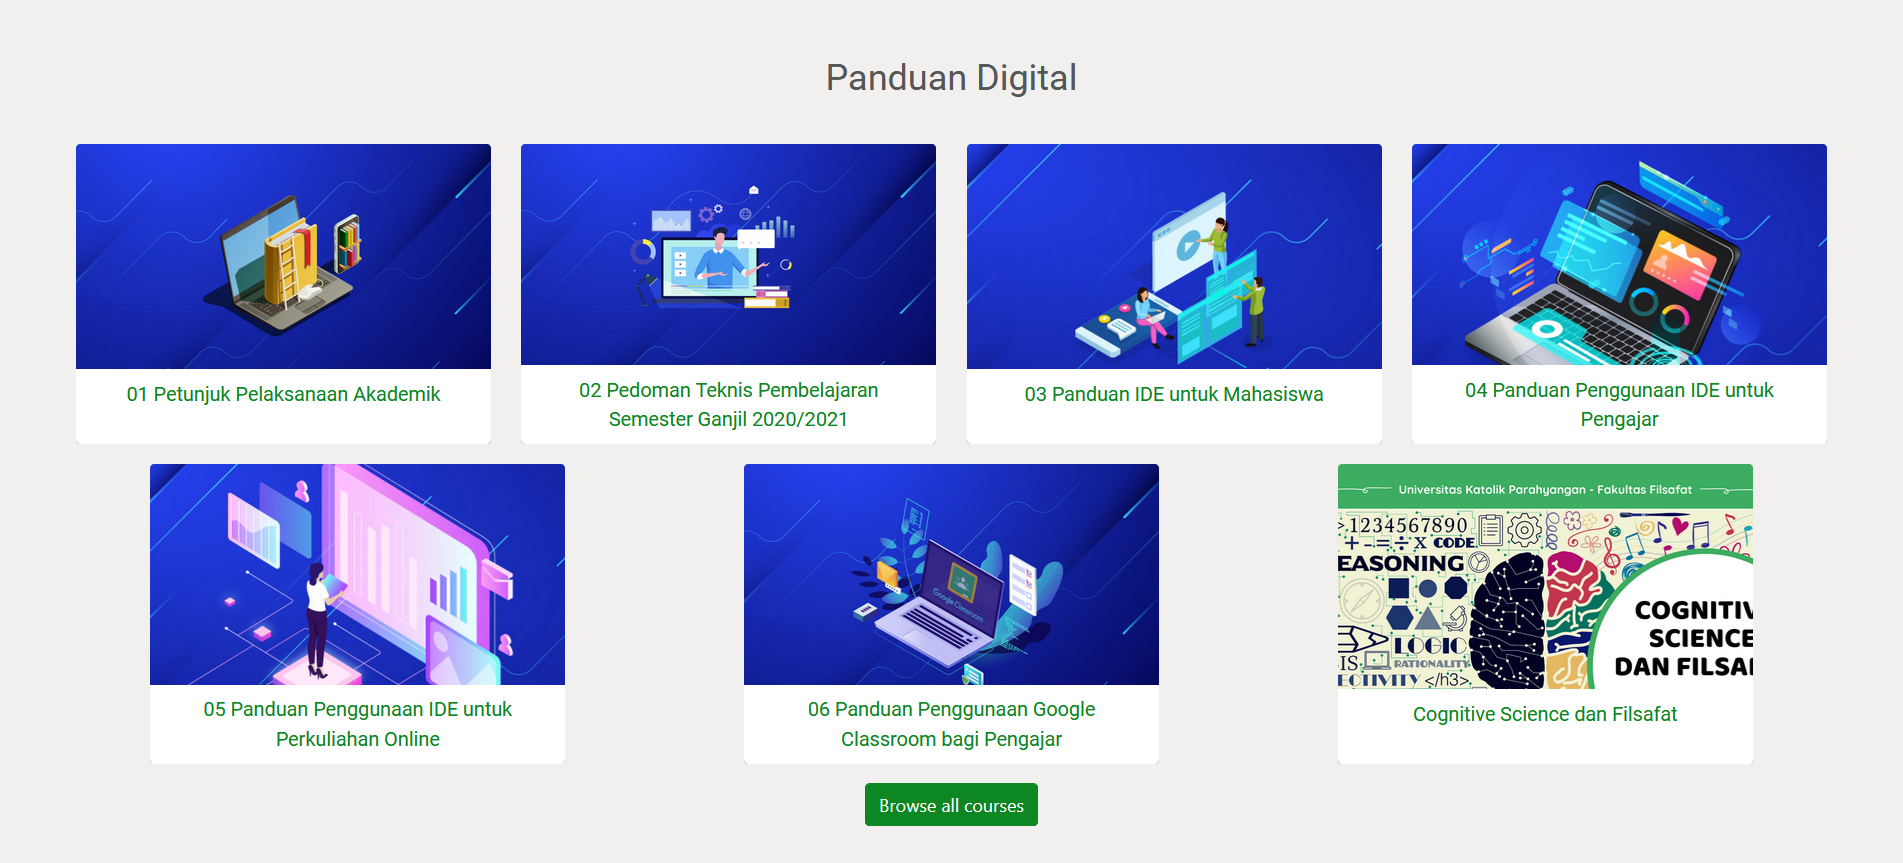
\includegraphics[scale=0.2]{panduan-digital.png}  
	\caption[Bagian panduan digital] {Bagian panduan digital pada halaman utama IDE UNPAR} 
	\label{fig:panduan-digital} 
\end{figure} 
\subsubsection {Video YouTube tersemat}
Halaman utama IDE memilik vidio YouTube yang tersemat berjudulkan "Tutorial IDE Mahasiswa".
\subsubsection {Branding UNPAR}
Branding yang dimaksud adalah penggunaan logo IDE UNPAR, nama IDE UNPAR dan skema warna yang berbeda dari skema warna milik Moodle dan skema warna bawaan tema Snap.
\subsubsection {SSO}
IDE UNPAR menggunakan SSO UNPAR untuk menangani pengguna yang ingin masuk ke dalam IDE UNPAR. Tombol \textit{login} pada halaman utama akan mengarahkan pengguna ke halaman SSO UNPAR seperti pada Gambar \ref{fig:sso-unpar} untuk memasukkan kredensial mereka.
\begin{figure}[H] 
	\centering  
	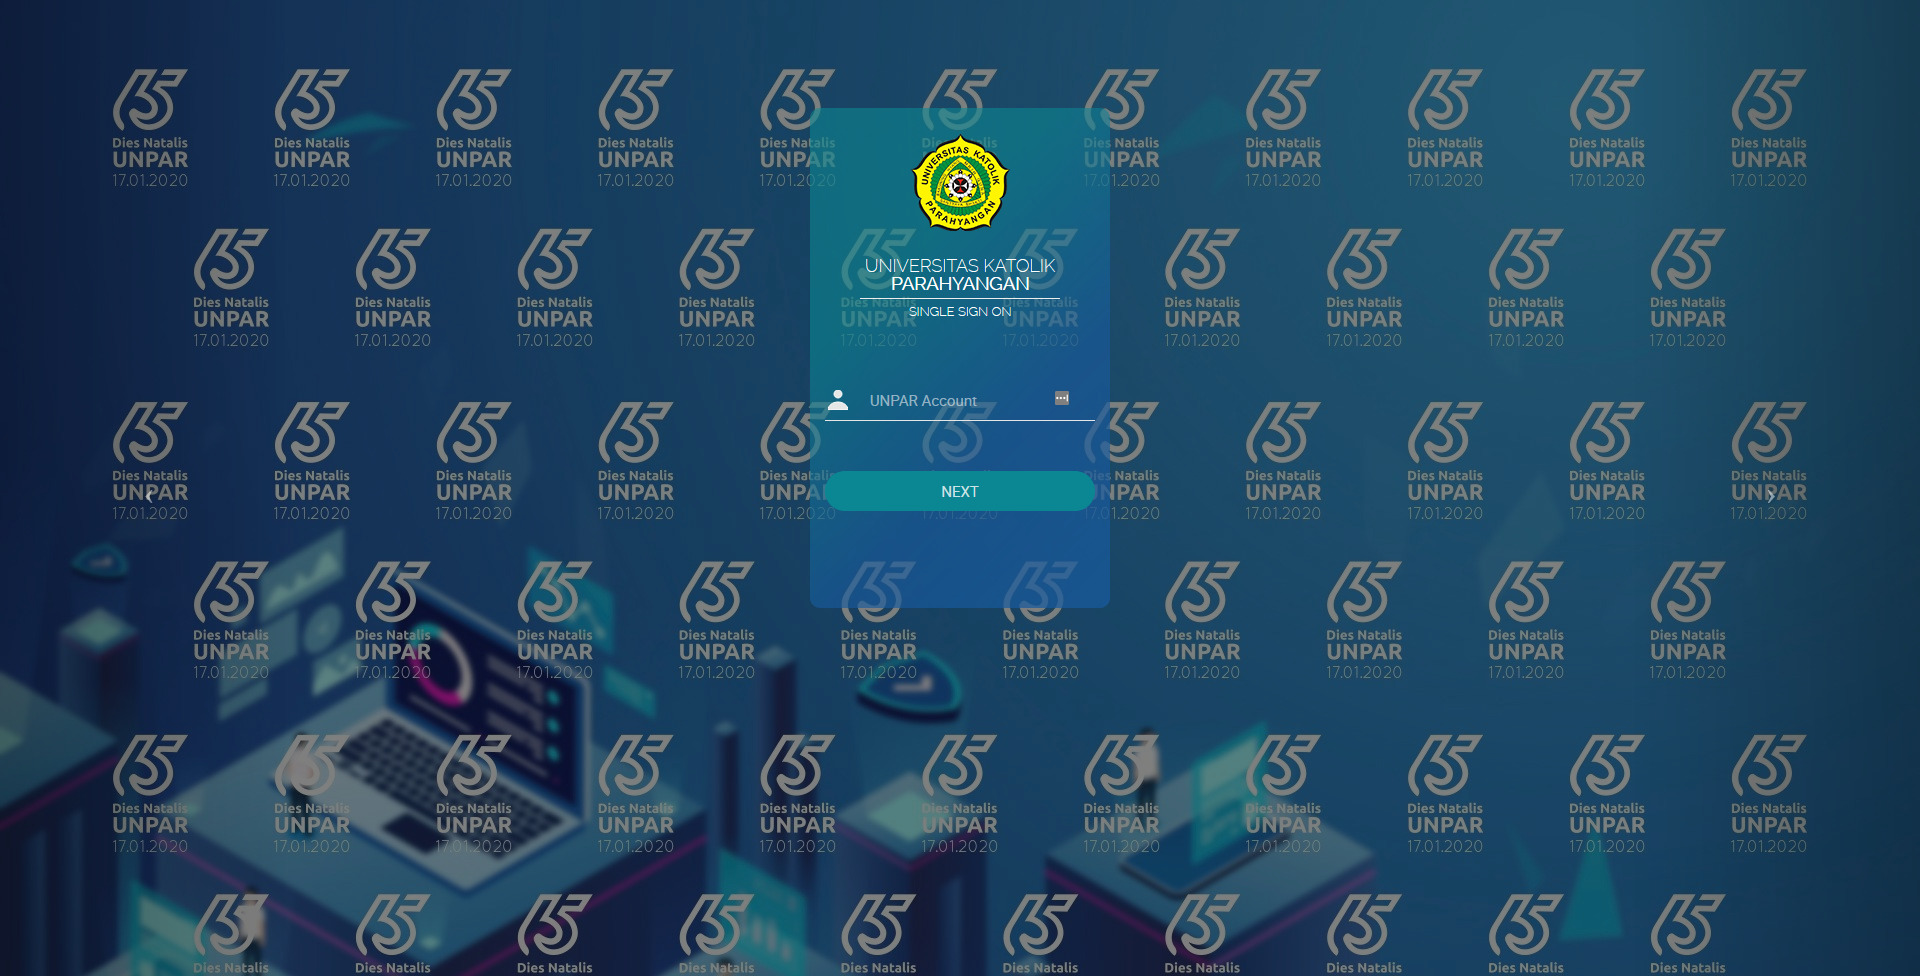
\includegraphics[scale=0.2]{sso-unpar.png}  
	\caption[Halaman SSO UNPAR] {Halaman SSO UNPAR} 
	\label{fig:sso-unpar} 
\end{figure} 

%tidak dapat digunakannya akses ke IDE UNPAR maka penilitian ini akan menggunakan sebuah situs demo yang dibuat dengan Moodle atau Moodle demo.

\section{Moodle demo (sementara)}

Pada saat dimulainya penulisan skripsi, penulis tidak dapat menghubungkan Moodle mobile dengan IDE UNPAR. Kesulitan menghubungkan Moodle mobile dengan IDE UNPAR terjadi ketika pengguna aplikasi diharuskan \textit{login} ke dalam IDE UNPAR melalui Moodle mobile dengan menggunakan SSO UNPAR. Moodle mobile tidak dapa sama sekali mengakses halaman SSO UNPAR. Sehingga untuk mengatasi masalah tersebut dibuatlah situs untuk mensimulasikan IDE UNPAR dengan URL \url{https://moodledemo.pascal.id} yang akan disebut sebagai Moodle demo.

Moodle demo dengan \textit{URL} \url{https://moodledemo.pascal.id} adalah situs demo yang akan digunakan. Moodle demo akan berfungsi sebagai \textit{web service} yang diakses oleh Moodle mobile. Sehingga Moodle demo akan menyimpan data mahasiswa, dosen, mata kuliah dan \textit{plugin} yang  ada pada IDE UNPAR untuk digunakan di dalam Moodle mobile. 
\subsection{Mata kuliah dan peserta mata kuliah}

Data yang berada pada Moodle demo berasal dari mata kuliah yang ada di IDE UNPAR diberikan oleh pembimbing, sehingga pada data mata kuliah tersebut terdapat bahan dan tugas. Peserta dari mata kuliah tersebut dibuat dengan sendiri mengikuti format penamaan yang berada di IDE UNPAR dan ada tiga peserta yang diikutkan dalam mata kuliah tersebut dengan tiga role yang berbeda yaitu \textit{teacher} yang dianggap seabagai dosen, \textit{non-editing teacher} dianggap sebagai asisten dosen dan \textit{student} dianggap sebagai mahasiswa.

\subsection{\textit{Plugin} dan tema}

\textit{Plugin} yang digunakan oleh Moodle demo adalah plugin standar Moodle karena pada IDE UNPAR tidak ditemukannya \textit{plugin} tambahan selain tema yang digunakan. \textit{Plugin} tema tidak harus digunakan karena tidak mempengaruhi Moodle mobile, namun dengan tujuan mengimitasi IDE UNPAR tema akan tetap digunakan karena peletakan \textit{banner}, video YouTube tersemat dan bagian panduan digital bergantung pada tema yang digunakan oleh IDE UNPAR. Tema pada situs moodle dapat dipasang dengan memasukkan file tema yang diambil dari situs \url{https://moodle.org/plugins/} ke dalam folder \texttt{/moodle/theme}. Setelah file berada dalam folder tersebut maka pada situs Moodle dibagian \textit{themes} akan muncul opsi tema yang baru saja dimasukkan.

Korsel pada untuk Moodle demo dapat dipasang dengan mengakses halaman menu tema. Pada halaman tersebut pilih opsi \textit{Cover display}, dalam opsi tersebut akan ada bagian untuk mengaktifkan dan memasang korsel untuk situs Moodle. Jumlah maksimal koresel yang dapat dipasang adalah 3 korsel. Korsel pada moodle demo ini bertujuan untuk mengimitasi \textit{banner} yang berada pada IDE UNPAR.

Bagian panduan digital pada IDE UNPAR adalah bagian \textit{featured course} yang diubah judulnya menjadi "panduan digital". Menggunakan fitur ini pada Moodle demo dapat dilakukan dengan mengakses halaman menu tema seperti pada Gambar \ref{fig:featured courses}, dan memilih opsi \textit{featured course} pada halaman tersebut. Jumlah \textit{course} maksimal yang dapat ditampilkan adalah 8. Karena peniliti tidak memiliki akses untuk \textit{course} panduan digital IDE, maka \textit{course} yang ditampilkan adalah \textit{course} yang sudah dimasukkan. Perubahan yang terjadi disini tidak akan terimplementasi dalam Moodle mobile.

\begin{figure}[H] 
	\centering  
	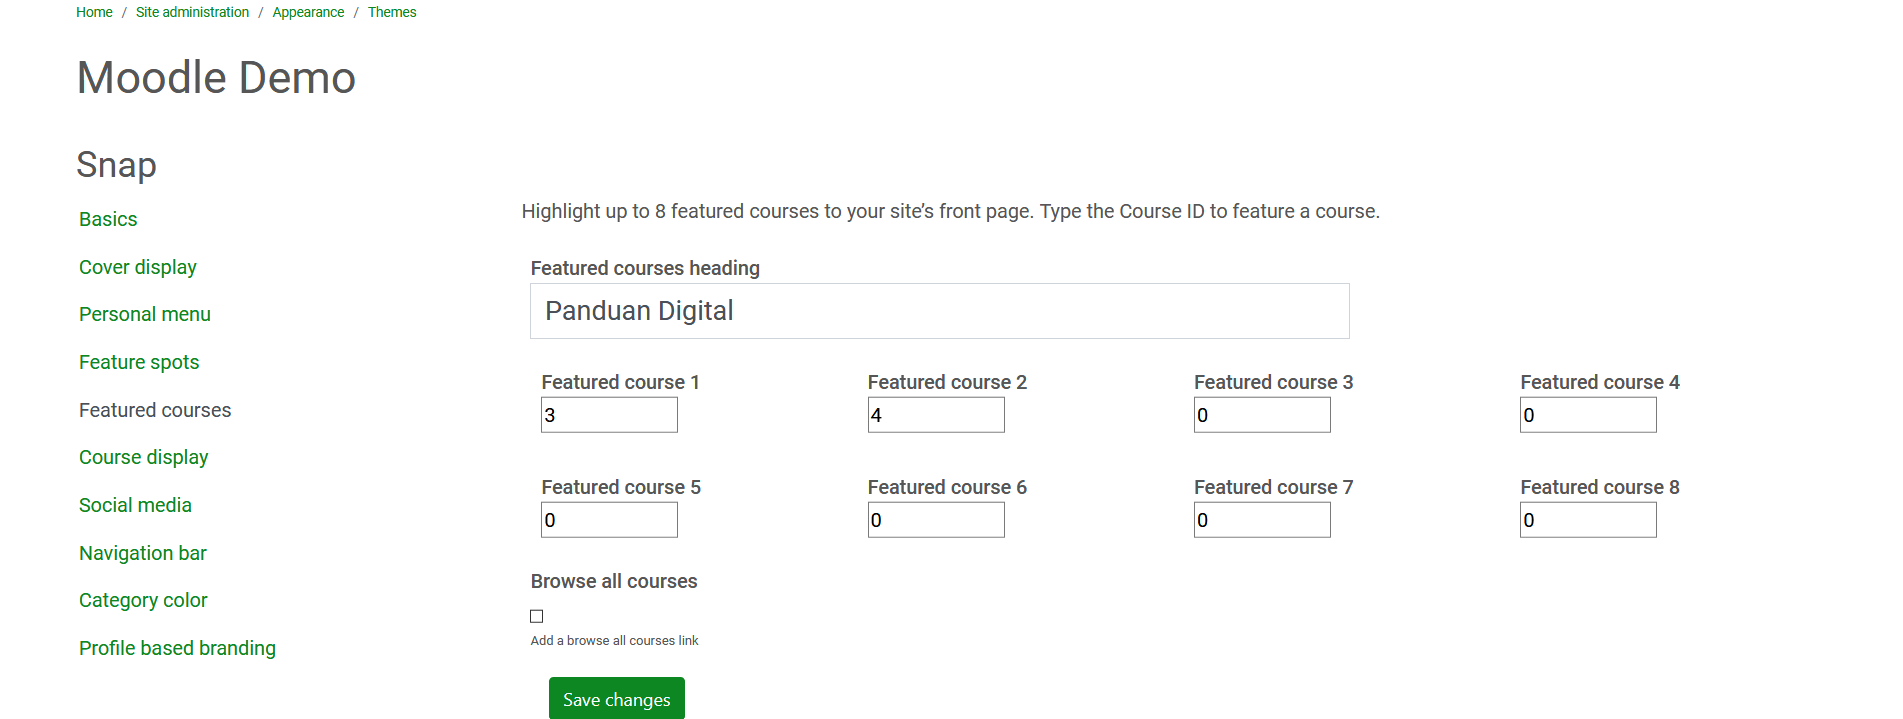
\includegraphics[scale=0.16]{featured-courses.png}  
	\caption[Halaman \textit{Featured Courses}] {Halaman \textit{Featured Courses}} 
	\label{fig:featured courses} 
\end{figure} 


Menambahkan sematan video YouTube dapat dikaukan dengan menekan tombol ikon roda gigi, kemudian memilih opsi \textit{turn editing on}. Dalam mode pengeditan tekan ikon kertas dan pensil seperti pada Gambar \ref{fig:editingmode}. Pada halaman edit, masukkan tag \textit{iframe} HTML dengan link video untuk menyematkannya. Seluruh perubahan yang dilakukan dalam mode pengeditan Moodle demo akan langsung terimplementasi juga pada Moodle mobile dalam halaman yang sesuai.

\begin{figure}[H] 
	\centering  
	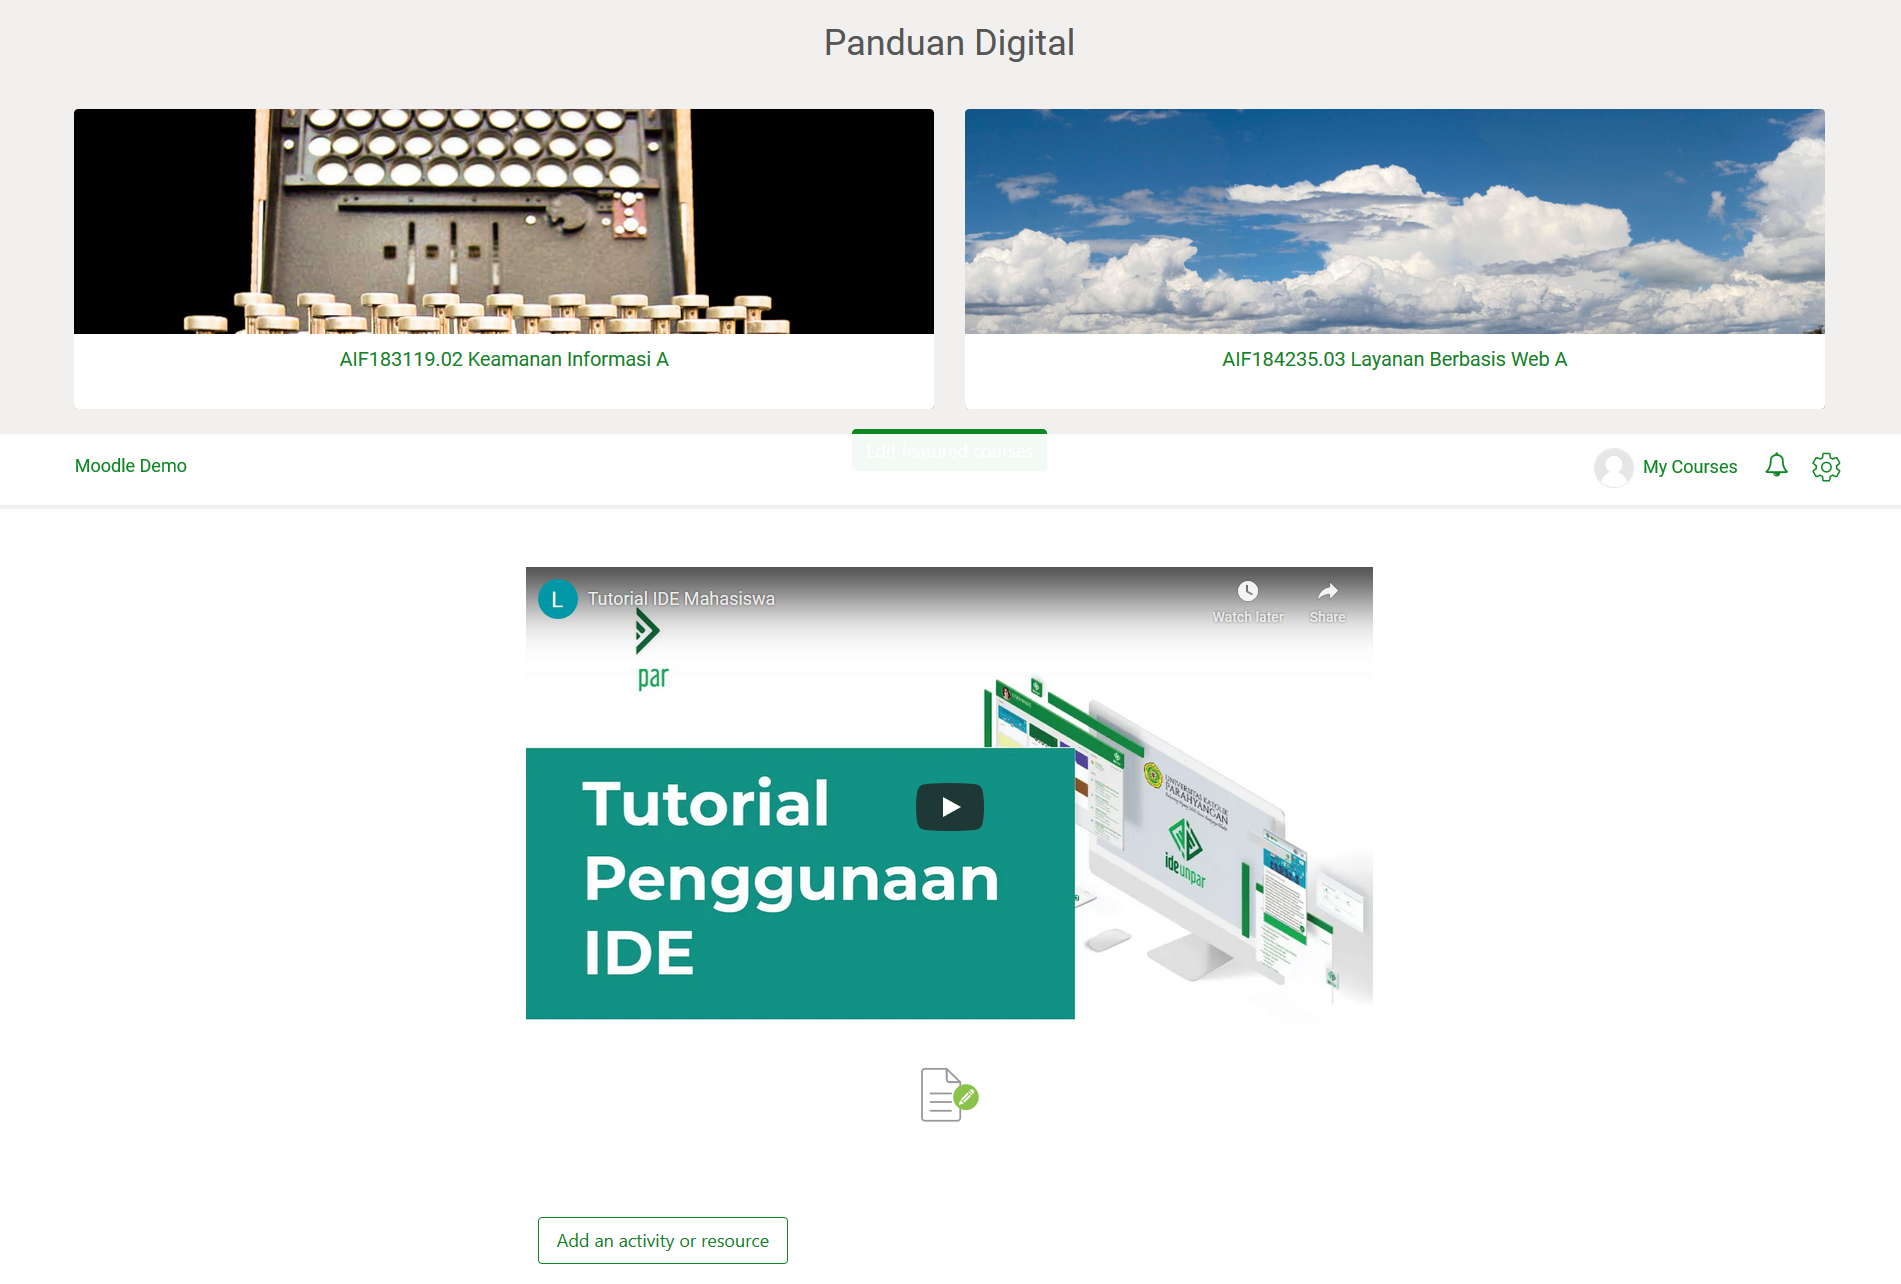
\includegraphics[scale=0.16]{demo-edit-mode.png}  
	\caption[Mode pengeditan] {Mode pengeditan} 
	\label{fig:editingmode} 
\end{figure} 

\subsection{Penyesuaian Moodle Mobile dengan IDE UNPAR}
Perubahan dan penyesuaian yang dibahas di \ref{sec:Kondisi IDE UNPAR} tidak semua dapat diterapkan ke dalam Moodle mobile. Penggunaan tema Snap dapat dilakukan dikarenakan Moodle mobile sudah tidak lagi mengukung penggunaan tema. Sehingga tampilan pada Moodle mobile akan diubah dengan mengubah \textit{source code}. \textit{Banner} pada halaman utama, bagian panduan digital dan branding UNPAR juga akan dilakukan dengan mengubah \textit{source code}, karena pada situs IDE UNPAR perubahan dan penyesuaian tersebut dilakukan pada tema yang digunakan. SSO juga tidak akan digunakan karena peneliti tidak memiliki akses SSO UNPAR.

Moodle mobile memungkinkan untuk mengatur \textit{URL preset} agar saat Moodle mobile dijalnkan, akan langsung diahlikan ke \textit{URL} tersebut. Namun ketika \textit{URL} IDE UNPAR digunakan terdapat \textit{error} dimana variable \texttt{\$urlscheme} memiliki nilai variable yang sudah diubah, dimana seharusnya variable tersebut berisi \texttt{moodlemobile://token=...} melainkan berisi \texttt{ide.unpar.ac.id://token=....}. Mengubah variable \texttt{urlscheme} pada Moodle mobile tetap tidak memungkinkan  IDE UNPAR diakses melalui Moodle mobile. Karena  adanya konfigurasi yang tidak dapat diakses untuk menghubungkan IDE UNPAR maka situs demo akan digunakan.

\section{Terhubungnya Moodle Mobile dengan IDE UNPAR}
\label{mobile:to:ide}

Pada tanggal 7 Maret 2021, Moodle mobile yang berada pada Google PlayStore dapat dihubungkan dengan situs IDE UNPAR. Dengan pengetahuan tersebut penulis mencoba kembali untuk menghubungkan Moodle mobile yang berada dalam mesin penulis dengan situs IDE UNPAR. Dengan pengaturan tersebut Moodle mobile pada mesin penulis dapat terhubung dengan IDE UNPAR, namun hanya dalam perangkat bergerak. Ketika dilakukan uji coba menghubungkan pada browser terdapat pesan \textit{error} seperti pada Gambar \ref{fig:protocolerror}. Sehingga pengujian aplikasi selama pengembangan akan dilakukan menggunakan perangkat bergerak.

\begin{figure}[H] 
	\centering  
	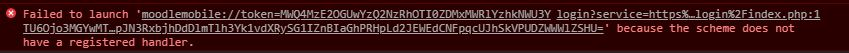
\includegraphics[scale=0.5]{scheme-has-no-handler.jpg}  
	\caption[Pesan pada Console browser] {Pesan pada console browser} 
	\label{fig:protocolerror} 
\end{figure} 

\section{Lisensi Moodle mobile}

Moodle mobile dilisensikan dengan lisensi \textit{Apache 2.0}\cite{Moodlemobile:license}. Lisensi tersebut mengizinkan untuk melakukan reproduksi dari Moodle mobile dengan atau tanpa modifikasi. Seperti yang disebut pada poin 4 lisesnsi dengan judul \textit{"Redistribution"}, hal-hal tersebut dapat dilakukan apabila memenuhi syarat-syarat yang tertera. Syarat-syarat yang dimaksud adalah :
\begin{itemize}
\item Aplikasi yang dibuat harus disertakan dengan salinan lisensi \textit{Apcahe 2.0}.
\item Seluruh file yang dimodifikasi harus menyertakan pemberitahuan yang jelas bahwa file tersebut sudah dimodifikasi.
\item Seluruh paten, \textit{trademark}, \textit{copyright} dan pemberitahuan atribusi harus disimpan dalam bentuk sumber untuk seluruh aplikasi yang akan didistrubusikan.
\item Apabila aplikasi sumber menyertakan file teks dengan judul \textit{\textbf{NOTICES}}, maka selurh aplikasi yang akan didistribusikan harus menyertakan salinan yang dapat dibaca.
\end{itemize}
Gagal memenuhi syarat-syarat di atas akan mengakibatkan lisensi untuk aplikasi yang telah dimodifikasi dan didistribusikan berrsifat tidak sah.

\section{Saran Fitur-fitur dari Umpan Balik}
\label{feature feedback}

Pada tanggal 25 Maret 2021 penguji membuat sebuah kuesioner yang dibagikan kepada warga UNPAR yang memiliki tautan untuk menguji coba aplikasi IDE UNPAR Mobile, kuesioner dapat dilihat pada \hyperref[lamp:B]{Lampiran B}. Form tersebut berisi pertanyaan yang menyangkut bagaimana pengalaman penggunaan aplikasi dan fitur-fitur apa saja yang mereka inginkan untuk diimplementasi. Tabel \ref{fitur yang diinginkan} adalah fitur-fitur yang diinginkan oleh penguji untuk diimplementasikan dan mungkin atau tidaknya untuk diimplementasikan.

\begin{table}[ht]
\caption{Hasil kuesioner untuk fitur apa yang diinginkan}
\centering
\resizebox{\textwidth}{!}{
\begin{tabular}{|l | l| c | c|}
\hline
\multicolumn{1}{|l|}{\multirow{2}{*}{Fitur yang ingin diimplementasikan}} & \multicolumn{1}{|l|}{\multirow{2}{*}{Sudah terimplementasi}} & \multicolumn{2}{|l|}{Dapat diimplementasikan?} \\ 
\cline{3-4}  
\multicolumn{1}{|l|}{} & \multicolumn{1}{|l|}{} &\multicolumn{1}{l|}{Ya} & \multicolumn{1}{l|}{Tidak} \\ \hline
Push notification  & \checkmark & &  \\ \hline
Scanner untuk foto menjadi PDF&  &  \checkmark & \\ \hline
Sinkronisasi dengan google calendar& & & \checkmark \\ \hline
Melihat file-file seperti PDF dan PPT di IDE UNPAR  & \checkmark & &  \\ \hline
Absensi melalui IDE UNPAR& & \checkmark & \\ \hline
Fitur tambah file otomatis dari apps scanner& & \checkmark & \\ \hline
Jadwal Kuliah& & &\checkmark \\ \hline
Sign in SSO dalam app & & &  \checkmark \\ \hline 
Dapat berpindah page dengan swipe horizontal & & & \checkmark\\ \hline
Fitur pesan  berupa message di IDE  menjadi bentuk chat & \checkmark &  &  \\ \hline
login langsung di aplikasi& & & \checkmark \\
\hline
\end{tabular}}
\label{fitur yang diinginkan}
\end{table}

\subsection{Push notification}
\label{push notif}
Fitur ini ditandakan sebagai tidak dapat diimplementasikan karena fitur tersebut sudah ada didalam Moodle mobile. Pengguna sudah bisa mendapatkan notifikasi dari aplikasi Moodle mobile dan dapat mengaturnya dari aplikasi itu sendiri.

\subsection{Scanner untuk foto menjadi PDF} 
\label{PDF scanner}
Fitur ini dapat diimplementasikan dengan bantuan dari \textit{plugin} Cordova \texttt{cordova-plugin-document-scanner}. Dengan plugin tersebut gambar yang ditangkap melalui kamera perangkat pengguna akan dimasukkan ke dalam format HTML yang kemudian akan dikonversi ke format PDF. Setelah dikonversi file PDF tersebut akan langsung diunggah ke dalam \textit{private files} atau submisi tugas.

\subsection{Sinkronisasi dengan Google Calendar}
Fitur ini tidak dapat diimplementasikan karena renggang waktu yang tidak cukup, sehingga tidak ditemukannya cara yang optimal untuk menghubungkan kalender IDE UNPAR dengan kalender Google melalui aplikasi IDE UNPAR mobile.

\subsection{Melihat file-file seperti PDF dan PPT di IDE UNPAR}
Fitur ini tidak dapat diimplementasikan karena dirasa menu \textit{File} yang telah disediakan oleh Moodle mobile dapat memenuhi kegunaan tersebut. Pengguna juga sudah bisa mengakses file-file yang disediakan di dalam mata kuliah untuk diunduh.

\subsection{Absensi melalui IDE UNPAR} 
\label{absesnsi IDE}
Fitur akan diimplementasi  melalui bentuk menu yang akan mengarahkan pengguna ke Student Portal UNPAR. Implementasi tersebut karena absesni dilakukan di dalam Student Portal Unpar dan tidak adanya integrasi untuk Moodle app.

\subsection{Fitur tambah file otomatis dari apps scanner}
\label{scanner app}
Fitur ini serupa dan akan terimplementasi sama dengan yang dibahas di subbab \ref{PDF scanner}.

\subsection{Jadwal Kuliah}
Fitur ini tidak akan diimplementasikan, karena jadwal perkuliahan tidak diatur atau ditunjukkan ke dalam IDE UNPAR melainkan di dalam Student Portal.

\subsection{Sign in SSO dalam app}
\label{in app sign in}
Fitur ini tidak dapat diimplementasikan karena moodle tidak dapat menampilkan SSO UNPAR di dalam aplikasinya sehingga SSO UNPAR tetap harus diakses melalui \textit{browser}. Fitur ini juga dirasakan tidak perlu karena Moodle mobile akan langsung mengarahkan kembali ke dalam aplikasi setalah berhasil login melalui \textit{browser}.

\subsection{Dapat berpindah page dengan swipe horizontal}
 \label{horizontal swipe}
 Fitur ini tidak akan diimplementasikan karena tidak cukupnya waktu untuk mengimplementasi fitur.

\subsection{Fitur Pesan yang berupa message di IDE di konversi menjadi bentuk chat }
\label{chat}
Fitur ini tidak diimplementasikan karena Moodle mobile sudah menunjukkan \textit{message} dalam bentuk \textit{chat}.

\subsection{Login langsung di aplikasi}
 \label{in app login}
Fitur ini tidak akan diimplementasi dengan alasan sama dengan yang dibahas di subbab \ref{in app sign in}.

